\section{Analisi Funzionale}%
\label{sec:analisi_funzionale}

\subsection{Sito Web}%
\label{sub:sito_web}

Il sito web pu\`o essere implementato usando qualsiasi framework, sarebbe ideale utilizzare framework con rendering veloce e la dimensione delle librerie non \`e importante siccome possono essere salvate integralmente in cache. Ho deciso di utilizzare React non necessariamente perch\`e \`e dotata delle suddette caratteristiche ma perch\`e ho avuto esperienza personale con il framework. Anche utilizzare vanilla Javascript per il rendering \`e possibile senza particolare complessit\`a.

Sar\`a necessario aggiungere i manifesti iOS e Android per permettere l'installazione del sito web come applicazione Progressive Web App.

\subsection{API}%
\label{sub:api}

La maggior parte delle web API di questo millennio hanno utilizzato la tecnologia REST (Representational state transfer), che associa ogni richiesta GET ad un'informazione e ogni richiesta POST, PUT, PATCH o DELETE ad un'azione, negli ultimi anni per\`o, le applicazioni web hanno iniziato ad introdurre numerose informazioni su singole pagine e la metodologia REST non scala con il numero di informazioni, infatti per ogni informazione l'utente deve inviare una nuova richiesta al server API\@. Per ovviare a questo problema \`e nato GraphQL\@.

GraphQL permette di richiedere solo le informazioni necessarie, riducendo le informazioni superflue ricevute in risposta dal server, inoltre permette di richiedere pi\`u informazioni insieme, ad esempio non \`e necessario ottenere prima le informazioni sulla spiaggia e poi i posti disponibili ma \`e possibile richiedere entrambe le informazioni nello stesso momento e anche per pi\`u spiaggie alla volta, riducendo il numero di richieste da centinaia ad una sola. % Bib: https://graphql.org/

Quindi la scelta della tipologia di API ricade su GraphQL ma le scelte non finiscono qui, infatti ora \`e necessario scegliere il linguaggio di programmazione da utilizzare per l'implementazione del servizio GraphQL\@. Sono disponibili librerie per ogni linguaggio ma ho deciso di utilizzare la libreria \href{https://github.com/graphql-rust/juniper}{Juniper} nel linguaggio Rust.

Rust \`e un linguaggio sviluppato da Mozilla con enfasi sulla sicurezza e sulla velocit\`a. Raggiunge velocit\`a equivalenti o superiori al linguaggio C ma le regole del linguaggio impediscono categoricamente la maggior parte delle vulnerabilit\`a ricorrenti nel linguaggio C\@. Lo sviluppo di applicazioni Rust non \`e semplice rispetto a linguaggi moderni come C\# e Javascript tuttavia la sua velocit\`a e la sua affidabilit\`a non \`e neanche confrontabile con questi linguaggi. % TODO: Bib: rust-lang

Rust riesce ad ottenere questa sicurezza tramite le restrizioni sull'utilizzo della memoria, infatti puntatori nulli o invalidi non sono permessi e non \`e possibile incorrere in \emph{race conditions}, inoltre non \`e presente un \emph{Garbage Collector} all'interno di Rust, le risorse sono acquisite durante l'inizializzazione e liberate quando escono fuori dallo \emph{scope}.

\subsection{Sicurezza informatica}%
\label{sub:sicurezza_informatica}

Per prevenire attacchi informatici di tipo DDoS (Distributed Denial of Service) ho scelto di utilizzare Cloudflare, un servizio che individua e filtra il traffico malevolo tramite l'analisi di tutte le richieste al server web. Cloudflare permette di analizzare le fonti di traffico e offre numerose statistiche utilizzabili dall'azienda per fidelizzare i clienti. Ci sono vari pacchetti di funzionalit\`a a prezzi differenti che dovrebbero essere presentati all'azienda cliente con i vari vantaggi e svantaggi. Per questo servizio il pacchetto gratuito \`e sufficiente ma \`e consigliabile il pacchetto \emph{Pro}. Cloudflare \`e l'azienda leader nell'ambito della protezione da attacchi DDoS, la sua rete ha la capacit\`a di 67 terabit per secondo, capace di bloccare tutti gli attacchi DDoS comuni. % bib: https://www.cloudflare.com/ddos/ && The Forrester Wave™: DDoS Mitigation Solutions, Q1 2021

Tra le varie funzionalit\`a offerte da Cloudflare troviamo certificati SSL gratuiti. Cloudflare offre diverse modalit\`a di configurazione dei certificati, siccome si pone tra i visitatori e il server web ci sono due tratte da proteggere, in automatico Cloudflare protegge la comunicazione tra i visitatori e Cloudflare tuttavia questo livello di protezione \`e molto ridotto, infatti se qualcuno riuscisse a intercettare il traffico tra Cloudflare e il server web, questo sarebbe in chiaro. Questo tipo di protezione prende il nome di \emph{Flexible SSL} ed \`e rivolto verso siti web che \textbf{non} trasmettono dati sensibili (Figura~\ref{fig:flexiblessl}) % Bib: https://www.cloudflare.com/ssl/

\begin{figure}[htpb]
    \centering
    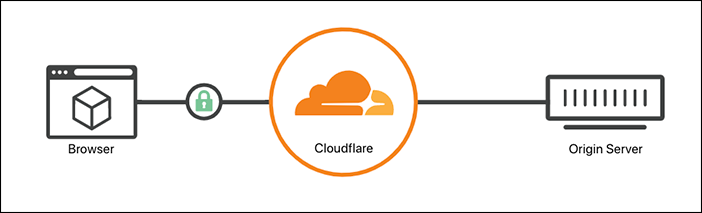
\includegraphics[width=0.8\linewidth]{cloudflare/flexible.png}
    \caption{Cloudflare con configurazione Flexible SSL}%
    \label{fig:flexiblessl}
\end{figure}

L'alternativa alle \emph{Flexible SSL} sono le \emph{Full SSL} (Figura~\ref{fig:fullssl}), queste aggiungono un secondo certificato tra Cloudflare \`e il sito web origine, il certificato pu\`o essere generato da Cloudflare gratuitamente, da Cerfication Authority oppure pu\`o essere generato localmente dall'azienda stessa. % Bib: https://support.cloudflare.com/hc/en-us/articles/200170416-End-to-end-HTTPS-with-Cloudflare-Part-3-SSL-options

\begin{figure}[htpb]
    \centering
    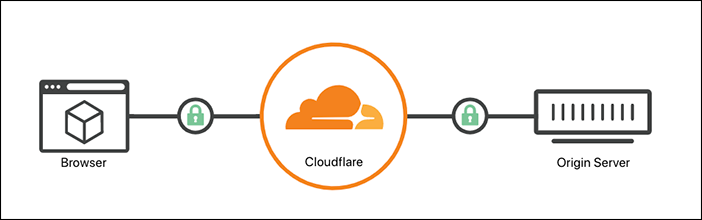
\includegraphics[width=0.8\linewidth]{cloudflare/full.png}
    \caption{Cloudflare con configurazione Full SSL}%
    \label{fig:fullssl}
\end{figure}

Il servizio per la prenotazione di spiaggie richiede l'utilizzo di Full SSL, tuttavia \`e richiesta completa fiducia verso Cloudflare: per permettere di individuare e filtrare i pacchetti malevoli, il traffico tra i visitatori e il server viene decifrato da Cloudflare e poi cryptato nuovamente con il secondo certificato. Cloudflare agisce come una VPN ad accesso remoto, il traffico viene cifrato tra il proxy e le sue fonti ma \textbf{il proxy ha accesso completo alle informazioni e pu\`o impersonare ogni utente}. Cloudflare \`e considerato affidabile dalle pi\`u grandi multinazionali del mondo ma \`e comunque necessario far presente di questa vulnerabilit\`a all'azienda. 

\subsection{Pagamento elettronico}%
\label{sub:pagamento_elettronico}

Per permettere ai clienti di prenotare spiaggie private \`e necessario implementare un servizio di e-commerce. Analizzando le varie possibilit\`a il servizio pi\`u adatto mi \`e sembrato essere \emph{PayPal Checkout}, le API sono semplici da integrare nel sito web e permette di pagare sia con PayPal che con carte di credito tuttavia richiede un account PayPal. Per semplificare il processo ho pianificato di distribuire la parte dovuta ad ogni spiaggia al termine del mese.